%\documentclass[handout]{beamer} 
\documentclass[t,12pt,numbers,fleqn]{beamer}
%\documentclass[ignorenonframetext]{beamer}

\newif\ifquestions
%\questionstrue
\questionsfalse

\usepackage{pgfpages} 
\usepackage{hyperref}
\hypersetup{colorlinks=true,
    linkcolor=blue,
    citecolor=blue,
    filecolor=blue,
    urlcolor=blue,
    unicode=false}
\urlstyle{same}

\usepackage{booktabs}
\usepackage{hhline}
\usepackage{multirow}
\usepackage{multicol}
\usepackage{array}

\usepackage{tikz}
\usetikzlibrary{positioning}

%\usepackage{natbib} %doesn't seem to work with beamer
\bibliographystyle{plain}
%\setcitestyle{authoryear}

%\usetheme{Iimenau}

\useoutertheme{split} %so the footline can be seen, without needing pgfpages

%\pgfpagesuselayout{resize to}[letterpaper,border shrink=5mm,landscape]  %if this is uncommented, the hyperref links do not work

\mode<presentation>{}

%% Requires:
%% 
%% \usepackage{latexsym}
%% \usepackage{amssymb}
%% \usepackage{stmaryrd}

%\renewcommand{\labelenumi}{(\theenumi)}

\newcommand{\be}{\begin{enumerate}}
\newcommand{\ee}{\end{enumerate}}
\newcommand{\bi}{\begin{itemize}}
\newcommand{\ei}{\end{itemize}}
\newcommand{\bc}{\begin{center}}
\newcommand{\ec}{\end{center}}
\newcommand{\bsp}{\begin{sloppypar}}
\newcommand{\esp}{\end{sloppypar}}

\newcommand{\sglsp}{\ }
\newcommand{\dblsp}{\ \ }

\newcommand{\iclicker}{i\texttt{>}clicker}

\newcommand{\sA}{\mbox{$\cal A$}}
\newcommand{\sB}{\mbox{$\cal B$}}
\newcommand{\sC}{\mbox{$\cal C$}}
\newcommand{\sD}{\mbox{$\cal D$}}
\newcommand{\sE}{\mbox{$\cal E$}}
\newcommand{\sF}{\mbox{$\cal F$}}
\newcommand{\sG}{\mbox{$\cal G$}}
\newcommand{\sH}{\mbox{$\cal H$}}
\newcommand{\sI}{\mbox{$\cal I$}}
\newcommand{\sJ}{\mbox{$\cal J$}}
\newcommand{\sK}{\mbox{$\cal K$}}
\newcommand{\sL}{\mbox{$\cal L$}}
\newcommand{\sM}{\mbox{$\cal M$}}
\newcommand{\sN}{\mbox{$\cal N$}}
\newcommand{\sO}{\mbox{$\cal O$}}
\newcommand{\sP}{\mbox{$\cal P$}}
\newcommand{\sQ}{\mbox{$\cal Q$}}
\newcommand{\sR}{\mbox{$\cal R$}}
\newcommand{\sS}{\mbox{$\cal S$}}
\newcommand{\sT}{\mbox{$\cal T$}}
\newcommand{\sU}{\mbox{$\cal U$}}
\newcommand{\sV}{\mbox{$\cal V$}}
\newcommand{\sW}{\mbox{$\cal W$}}
\newcommand{\sX}{\mbox{$\cal X$}}
\newcommand{\sY}{\mbox{$\cal Y$}}
\newcommand{\sZ}{\mbox{$\cal Z$}}

\renewcommand{\phi}{\varphi}
\newcommand{\seq}[1]{{\langle #1 \rangle}}
\newcommand{\set}[1]{{\{ #1 \}}}
\newcommand{\tuple}[1]{{( #1 )}}
\newcommand{\mlist}[1]{{[ #1 ]}}
\newcommand{\sembrack}[1]{\llbracket#1\rrbracket}
%\newcommand{\sembrack}[1]{[\![#1]\!]}
\newcommand{\synbrack}[1]{\ulcorner#1\urcorner}
\newcommand{\commabrack}[1]{\lfloor#1\rfloor}
\newcommand{\bsynbrack}[1]{\lceil#1\rceil}
\newcommand{\bsembrack}[1]{\lceil\!\!\lceil#1\rceil\!\!\rceil}
\newcommand{\mname}[1]{\mbox{\sf #1}}
\newcommand{\mcolon}{\mathrel:}
\newcommand{\mdot}{\mathrel.}
\newcommand{\modpar}{\models_{\rm par}}
\newcommand{\modreg}{\models_{\rm reg}}
\newcommand{\proves}[2]{#1 \vdash #2}
\newcommand{\notproves}[2]{#1 \not\vdash #2}
\newcommand{\provesin}[3]{#1 \vdash_{#2} #3}
\newcommand{\notprovesin}[3]{#1 \not\vdash_{#2} #3}
%\newcommand{\leqq}[1]{\mathrel{\preceq_{#1}}}
\newcommand{\parrow}{\rightharpoonup}
\newcommand{\tarrow}{\rightarrow}
\newcommand{\term}{\seq}
\newcommand{\lub}{\sqcup}
\newcommand{\subfun}{\sqsubseteq}
\newcommand{\subpred}{\subseteq}
\newcommand{\BoxApp}{\Box\,}
\newcommand{\BOX}{\mathrel{\Box}}
\newcommand{\funapp}{\mathrel@}

\newcommand{\com}{\mname{complement}}
\newcommand{\dom}{\mname{domain}}
\newcommand{\sumcl}{\mname{sum}}
\newcommand{\pow}{\mname{power}}
\newcommand{\pair}{\mname{pair}}
\newcommand{\opair}{\mname{ordered-pair}}
\newcommand{\inters}{\mname{intersection}}
\newcommand{\emp}{\mname{empty}}
\newcommand{\uni}{\mname{univocal}}
\newcommand{\fun}{\mname{function}}
\newcommand{\card}{\mname{card}}
\newcommand{\sets}{\mname{sets}}
\newcommand{\monotone}{\mname{monotone}}
\newcommand{\continuous}{\mname{continuous}}
\newcommand{\chain}{\mname{chain}}
\newcommand{\mub}{\mname{ub}}
\newcommand{\mlub}{\mname{lub}}
\newcommand{\fixedpoint}{\mname{fp}}
\newcommand{\leastfixedpoint}{\mname{lfp}}
\newcommand{\strongfixedpoint}{\mname{sfp}}
\newcommand{\emptyfun}{\triangle}
\newcommand{\statetrans}[1]{\stackrel{#1}{\longrightarrow}}
\newcommand{\thyext}{\leq}
\newcommand{\conthyext}{\unlhd}

\newcommand{\Iota}{\mbox{\rm I}}
\newcommand{\IotaApp}{\mbox{\rm I}\,}
\newcommand{\iotaApp}{\iota\,}
\newcommand{\epsilonApp}{\epsilon\,}
\newcommand{\True}{\mbox{\sf T}} 
\newcommand{\False}{\mbox{\sf F}} 
\newcommand{\Trueword}{\sf true}
\newcommand{\Falseword}{\sf false}
\newcommand{\Neg}{\neg} 
\newcommand{\Andd}{\wedge}
\newcommand{\Or}{\vee}
\newcommand{\Implies}{\supset}
\newcommand{\ImpliesAlt}{\Rightarrow}
\newcommand{\Iff}{\equiv}
\newcommand{\Sheffer}{\mathrel|}
\newcommand{\IffAlt}{\Leftrightarrow}
\newcommand{\Forall}{\forall}
\newcommand{\ForallApp}{\forall\,}
\newcommand{\Forsome}{\exists}
\newcommand{\ForsomeApp}{\exists\,}
\newcommand{\ForsomeUniqueApp}{\exists\,!\,}
\newcommand{\IsDef}{\downarrow}
\newcommand{\IsUndef}{\uparrow}
\newcommand{\Equal}{=}
\newcommand{\QuasiEqual}{\simeq}
\newcommand{\Undefined}{\bot}
\newcommand{\If}{\mname{if}}
\newcommand{\IsDefApp}{\!\IsDef}
\newcommand{\IsUndefApp}{\!\IsUndef}
\newcommand{\TRUE}{\mbox{{\sc t}}}
\newcommand{\FALSE}{\mbox{{\sc f}}}
\newcommand{\truthvalues}{\{\TRUE,\FALSE\}}
\newcommand{\LambdaApp}{\lambda\,}
\newcommand{\LAMBDAapp}{\Lambda\,}
\newcommand{\AlphaEquiv}{\stackrel{\alpha}{=}}

\newcommand{\mvar}[3]{\textbf{var}_{#1}[#2,#3]}
\newcommand{\mterm}[2]{\textbf{term}_{#1}[#2]}
\newcommand{\mform}[2]{\textbf{form}_{#1}[#2]}
\newcommand{\mtype}[2]{\textbf{type}_{#1}[#2]}
\newcommand{\mexpr}[3]{\textbf{expr}_{#1}[#2,#3]}

\newcommand{\imps}{\mbox{\sc imps}}
\newcommand{\fol}{\mbox{\sc fol}}
\newcommand{\lutins}{\mbox{\sc lutins}}
\newcommand{\vlisp}{\mbox{\sc vlisp}}
\newcommand{\vmach}{\mbox{\sc vmach}}
\newcommand{\gnu}{\mbox{\sc gnu}}
\newcommand{\zf}{\mbox{\sc zf}}
\newcommand{\nbg}{\mbox{\sc nbg}}
\newcommand{\pnbg}{\mbox{\sc pnbg}}
\newcommand{\snbg}{\mbox{\sc snbg}}
\newcommand{\pfol}{\mbox{\sc pfol}}
\newcommand{\nbgstar}{$\mbox{\sc nbg}^\ast$}
\newcommand{\boldnbgstar}{$\mbox{\bf NBG}^\ast$}
\newcommand{\stt}{\mbox{\sc stt}}
\newcommand{\eves}{\mbox{\sc eves}}
\newcommand{\hol}{\mbox{\sc hol}}
\newcommand{\mizar}{Mizar}
\newcommand{\nqthm}{Nqthm}
\newcommand{\pvs}{\mbox{\sc pvs}}
\newcommand{\stmm}{\mbox{\sc stmm}}

\iffalse
\newtheorem{thm}{Theorem}[section]
\newtheorem{cor}[thm]{Corollary}
\newtheorem{lem}[thm]{Lemma}
\newtheorem{prop}[thm]{Proposition}
\newtheorem{rem}[thm]{Remark}
\newtheorem{eg}[thm]{Example}
\newtheorem{df}[thm]{Definition}
\fi

%\newenvironment{proof}{\par\noindent{\bf Proof\ \ }}{$\Box$}

\newenvironment{namedform}[1]
   {\begin{tabbing}\textbf{#1}\ }
   {\end{tabbing}}

\newcommand{\urlpart}[1]{\mbox{\texttt{#1}}\linebreak[0]}

\newcommand{\bblue}{\textcolor{blue!80!black}}
\newcommand{\bgreen}{\textcolor{green!55!black}}
\newcommand{\bbrown}{\textcolor{brown}}
\newcommand{\bred}{\textcolor{red!80!black}}
\newcommand{\bcyan}{\textcolor{cyan!80!black}}
\newcommand{\bmagenta}{\textcolor{magenta}}
\newcommand{\byellow}{\textcolor{yellow}}
\newcommand{\borange}{\textcolor{orange}}
\newcommand{\bviolet}{\textcolor{violet}}
\newcommand{\bpurple}{\textcolor{purple}}
\newcommand{\bdarkgray}{\textcolor{darkgray}}
\newcommand{\bgray}{\textcolor{gray}}
\newcommand{\blightgray}{\textcolor{lightgray}}

\newcommand{\clicker}{i\texttt{>}clicker}

\newenvironment{changemargin}[2]{%
  \begin{list}{}{%
    \setlength{\topsep}{0pt}%
    \setlength{\leftmargin}{#1}%
    \setlength{\rightmargin}{#2}%
    \setlength{\listparindent}{\parindent}%
    \setlength{\itemindent}{\parindent}%
    \setlength{\parsep}{\parskip}%
  }%
  \item[]}{\end{list}}


\newcommand{\topic}{02 Getting Started}

%Title page information for 1D04 lectures slides

% Define year specific parameters - used in title page and footer

\newcommand{\season}{Fall} %use to switch between Winter and Fall
\newcommand{\instructor}{Dr.~Spencer Smith} %use to switch instructor
\newcommand{\instructSmall}{Dr.~Smith}
\newcommand{\yr}{2017}
\newcommand{\courseCode}{CAS 741, CES 741}
\newcommand{\courseTitle}{Development of Scientific Computing Software}

%\setbeamerfont{structure}{series=\bfseries}
%\usefonttheme[stillsansseriftext,stillsansserifmath]{serif}
\setbeamertemplate{navigation symbols}{} 
\setbeamertemplate{itemize item}[ball]

\title{
  {\normalsize \bf 
    \borange{\courseCode~(\courseTitle)\\ \season~\yr}}\\[2ex]
  {\Large \bf \topic}}

\author[Smith]{\instructor}

\institute{
  Faculty of Engineering,
  McMaster University}

\date{
\today
%January 2011\\
\bc
  
\includegraphics[scale = 0.2, keepaspectratio]
  {../mcmaster-logo-full-color.jpg}
\ec
}

\renewcommand{\borange}[1] %orange is too hard to read
{
   \bred{#1}
}

\begin{document}

%\nobibliography{../../ReferenceMaterial/References}

% Footline for  Slides

% Display title page and displays footers

\setbeamertemplate{footline}{} %so the title screen does not have a footline

%%%%%%%%%%%%%%%%%%%%%%%%%%%%%%%%%%%%%%%%%%%%%%%%%%%%%%%%%%%%

\begin{frame}
\titlepage
\end{frame}

%%%%%%%%%%%%%%%%%%%%%%%%%%%%%%%%%%%%%%%%%%%%%%%%%%%%%%

\setbeamertemplate{footline}{
\begin{beamercolorbox}{sectioninhead/foot}
\hspace{1ex}\bblue{\hrulefill}\hspace{1ex}

\vspace{1ex}
\hspace{1ex}
{\tiny \instructSmall \hfill 
\courseCode~\season~\yr:~\topic \hfill 
\insertframenumber/\inserttotalframenumber~~}
%\insertframenumber/\ref{lastframe}}
%\hfill {\small \insertframenumber} \hspace{10ex}
%{\small $$\insertframenumber$$}
\vspace{1ex}
\end{beamercolorbox}}

%%%%%%%%%%%%%%%%%%%%%%%%%%%%%%%%%%%%%%%%%%%%%%%%%%%%%%


%%%%%%%%%%%%%%%%%%%%%%%%%%%%%%%%%%%%%%%%%%%%%%%%%%

\begin{frame}
\frametitle{Getting Started}

\bi
\item LiCS overview by Dan
\item Administrative details
\item Questions on suggested reading?
\item Project choices
\item Software tools
\item Software Engineering for Scientific Computing literature
\ei

\end{frame}

%%%%%%%%%%%%%%%%%%%%%%%%%%%%%%%%%%%%%%%%%%%%%%%%%%

\begin{frame}
\frametitle{Administrative Details}

\bi
\item Benches and white boards
\item Use folder structure given in repo
\item Post any questions as issues in our repo
\item Problem statement due Friday, Sept 15 by 11:59 pm
\ei

\end{frame}

%%%%%%%%%%%%%%%%%%%%%%%%%%%%%%%%%%%%%%%%%%%%%%%%%%

\begin{frame}
\frametitle{Benches and Glassboards}

\begin{tikzpicture}[remember picture,overlay]
\node [xshift=0cm,yshift=0.15cm] at (current page.center)
{
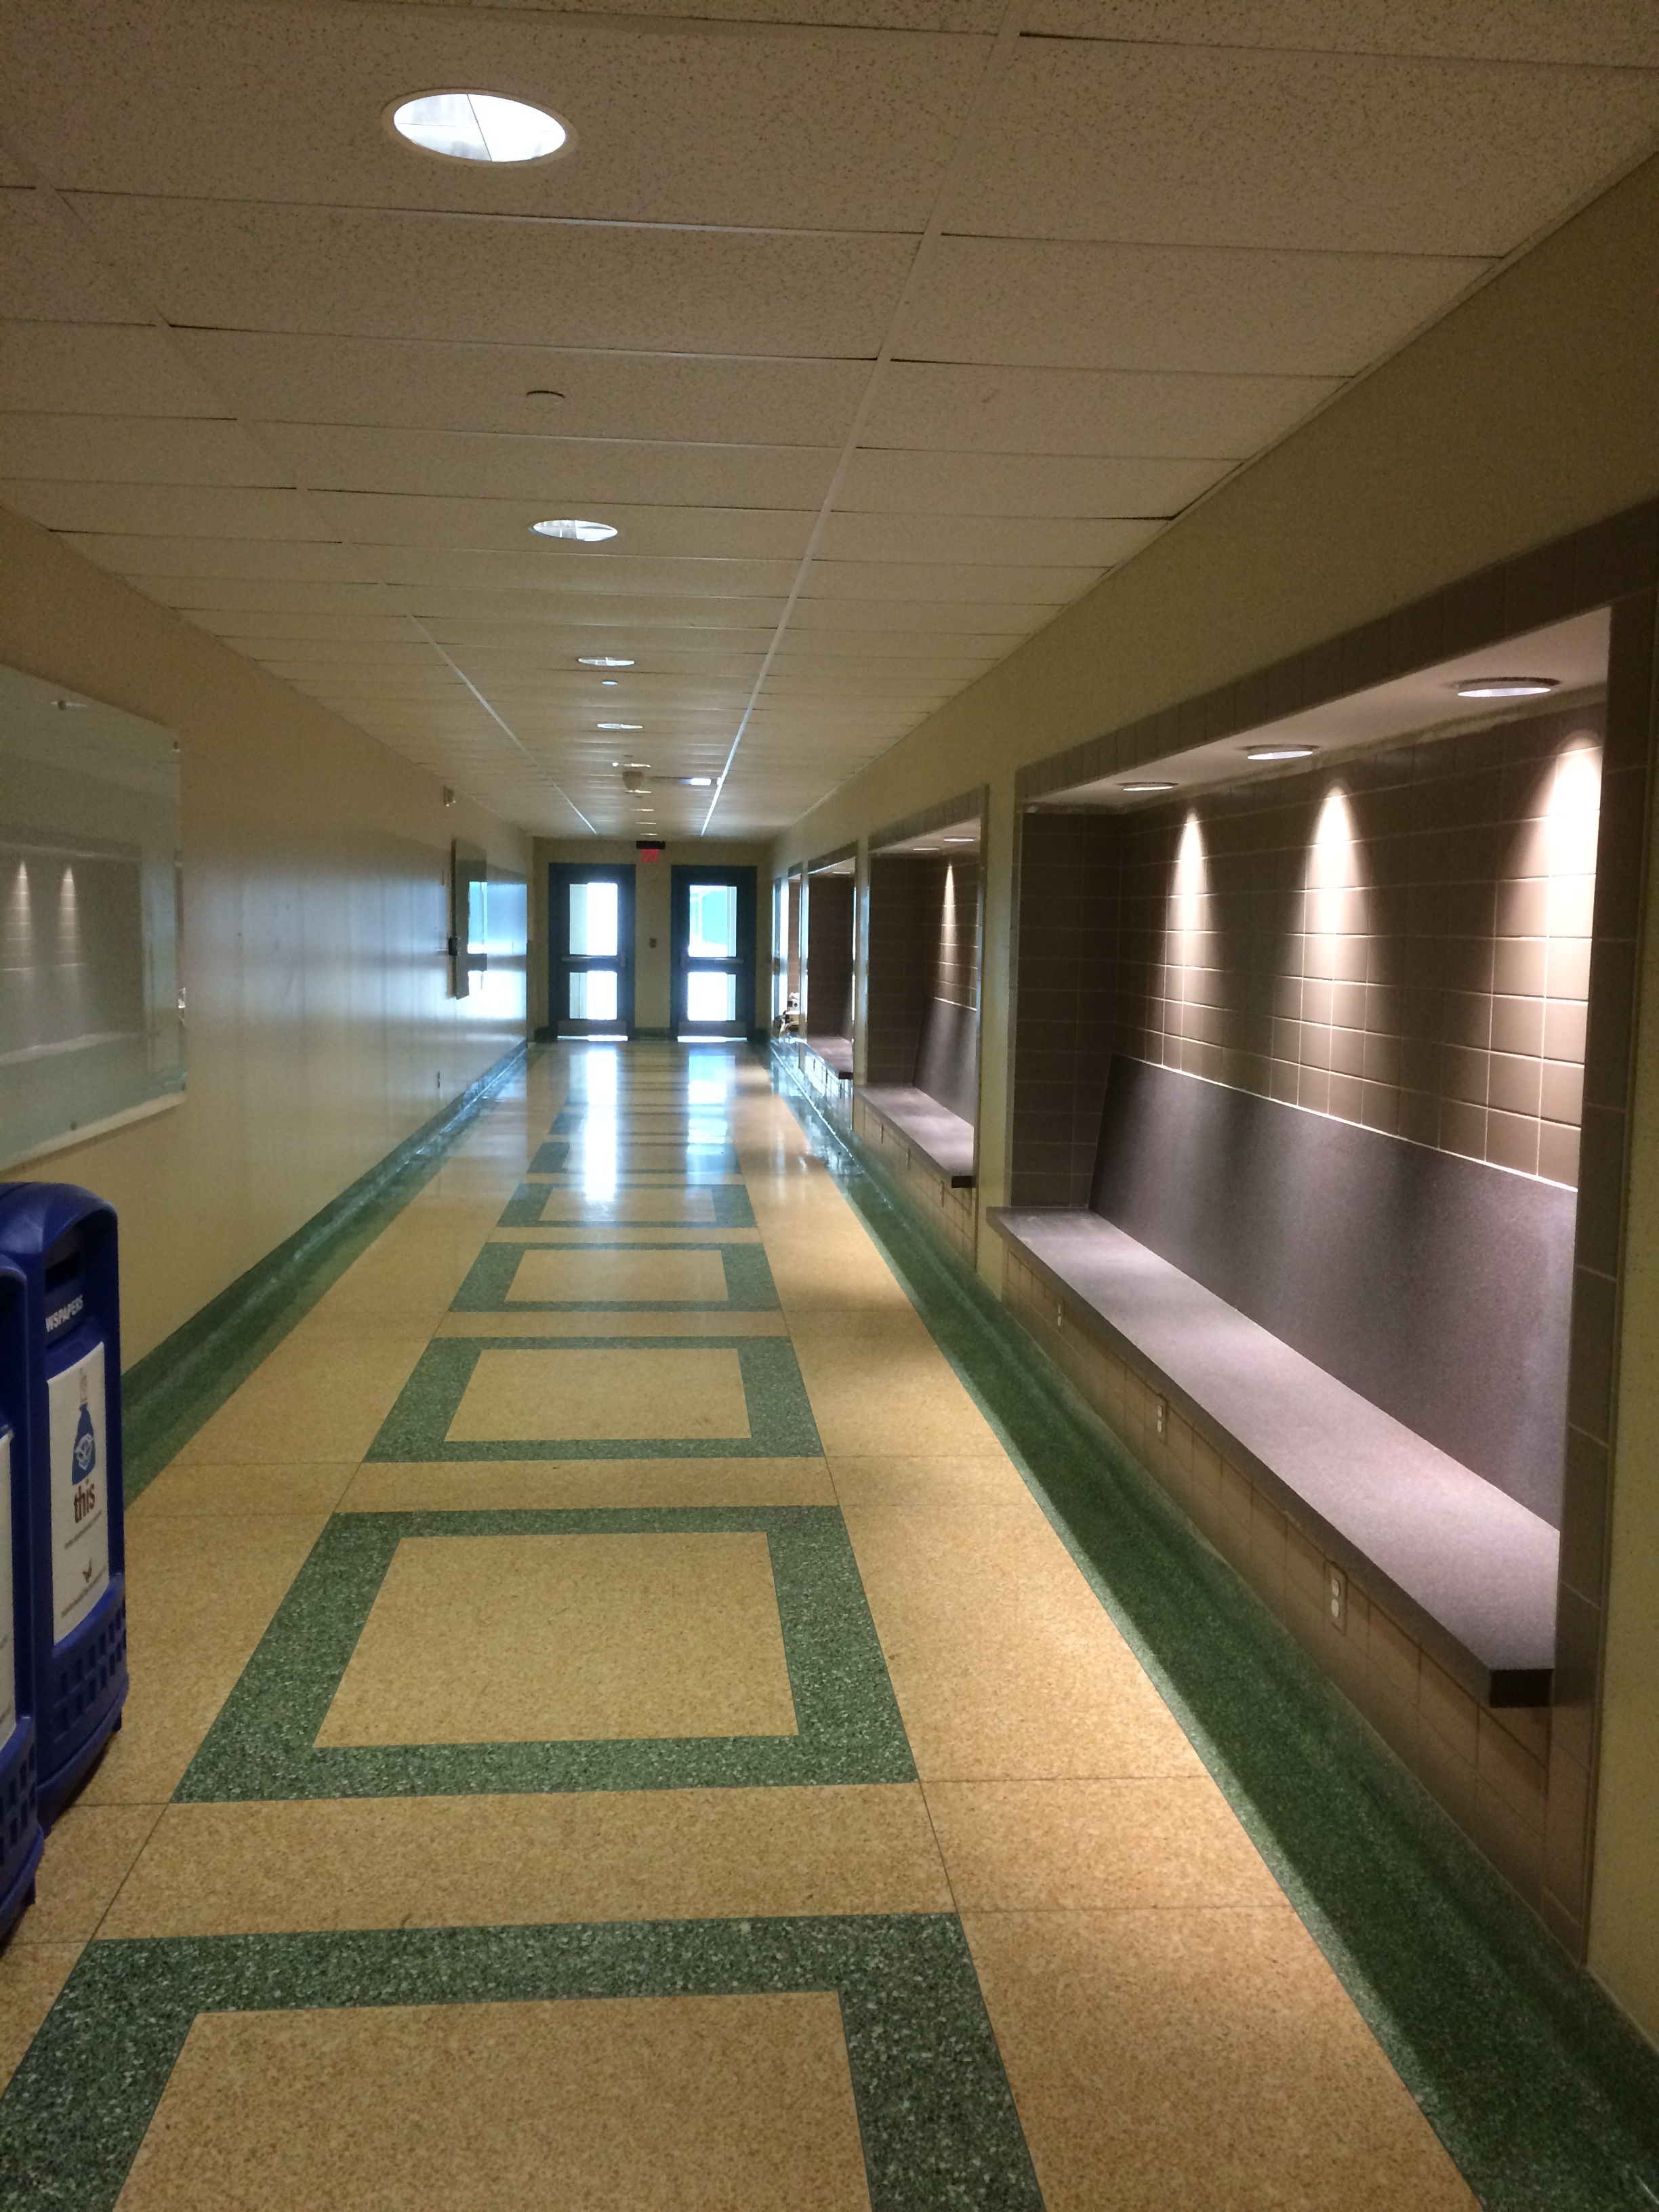
\includegraphics[width=0.5\textwidth]{../Figures/GlassBoards.jpg}
};
\end{tikzpicture}

\end{frame}

%%%%%%%%%%%%%%%%%%%%%%%%%%%%%%%%%%%%%%%%%%%%%%%%%%

\begin{frame}
\frametitle{Administrative Details: Grade Assessment}

\begin {enumerate}

\item Presentations and class discussion 10\%

\item Quality of GitHub issues provided to classmates 5\%

\item Problem Statement 0\%

\item System Requirements Specification (SRS) 20\%

\item Verification and Validation Plan 10\%

\item Module Guide (MG) 10\%

\item Module Interface Specification (MIS) 10\%

\item Final Documentation (including revised versions of previous documents,
  plus the source code and a testing report) 35\%

\end {enumerate}

\end{frame}

%%%%%%%%%%%%%%%%%%%%%%%%%%%%%%%%%%%%%%%%%%%%%%%%%%

\begin{frame}
\frametitle{Administrative Details: Report Deadlines}
~\newline
\begin{tabular}{l l l}
Problem Statement & Week 02 & Sept 15\\
System Requirements Specification (SRS) & Week 05 & Oct 4\\
Verification and Validation Plan & Week 07 & Oct 25\\
Module Guide (MG) & Week 09 & Nov 8\\
Module Interface Specification (MIS) & Week 11 & Nov 22\\
Final Documentation & Week 13 & Dec 6\\
\end {tabular}

\bi
\item The written deliverables will be graded based on the repo contents as of
11:59 pm of the due date
\item If you need an extension, please ask
\item Two days after each major deliverable, your GitHub issues will be due
\ei

\end{frame}

%%%%%%%%%%%%%%%%%%%%%%%%%%%%%%%%%%%%%%%%%%%%%%%%%%

\begin{frame}
\frametitle{Administrative Details: Presentations}

~\newline
\begin{tabular}{l l l}
SRS Present & Week 04 & Week of Sept 25\\
V\&V Present & Week 06 & Week of Oct 16\\
MG Present & Week 08 & Week of Oct 30\\
MIS Present & Week 10 & Week of Nov 13\\
Implementation Present & Week 12 & Week of Nov 27\\
\end {tabular}

\bi
\item Tentative dates
\item Specific schedule depends on final class registration and need
\item Informal presentations with the goal of improving everyone's written
  deliverables
\ei

\end{frame}

%%%%%%%%%%%%%%%%%%%%%%%%%%%%%%%%%%%%%%%%%%%%%%%%%%

\begin{frame}
\frametitle{Questions on Suggested Reading?}

\begin {itemize}

\item \href{https://gitlab.cas.mcmaster.ca/smiths/cas741/blob/master/ReferenceMaterial/SoftEngForScienceBook.pdf}{Smith2016~\cite{Smith2016}}
\item \href{https://gitlab.cas.mcmaster.ca/smiths/cas741/blob/master/ReferenceMaterial/SmithLaiAndKhedri2007fulltext.pdf}{SmithEtAl2007~\cite{SmithEtAl2007}}

\end{itemize}

\end{frame}

%%%%%%%%%%%%%%%%%%%%%%%%%%%%%%%%%%%%%%%%%%%%%%%%%%

\begin{frame}
\frametitle{Project Selection: Desired Qualities}
\begin{itemize}
\item Related to scientific computing
\item Simple, but not trivial
\item If feasible, select a project related to your research
\item Ideally, re-implement existing software
\item Each student project needs to be unique
\item Possibly a specific physical problem
\item Possibly a (family of) general purpose tool(s)
\item Some examples follow, the links are just places to get started
\end{itemize}
\end{frame}

%%%%%%%%%%%%%%%%%%%%%%%%%%%%%%%%%%%%%%%%%%%%%%%%%%

\begin{frame}
\frametitle{Project Selection: Specific Physical Problem}
\begin{itemize}
\item
  \href{https://ocw.mit.edu/courses/mathematics/18-303-linear-partial-differential-equations-fall-2006/lecture-notes/heateqni.pdf}{
    Heated
    rod}
\item \href{http://www.tech.plym.ac.uk/sme/THER204B-web/Heatran2.PDF}{Heated plate}
\item \href{https://en.wikipedia.org/wiki/Double_pendulum}{Double pendulum}
\item \href{http://chrishecker.com/Rigid_Body_Dynamics}{Rigid body dynamics}
\item Column buckling
\item \href{https://en.wikipedia.org/wiki/Harmonic_oscillator}{Damped harmonic oscillator}
\item Stoichiometric calculations (chemical balance)
\item
  \href{http://www.tiem.utk.edu/~gross/bioed/bealsmodules/predator-prey.html}{Predator
    prey dynamics}
\item Imaging: filters, edge detection etc.
\item etc.
\end{itemize}

\end{frame}

%%%%%%%%%%%%%%%%%%%%%%%%%%%%%%%%%%%%%%%%%%%%%%%%%%

\begin{frame}
\frametitle{Project Selection: Family of General Purpose Tools}
\begin{itemize}
\item \href{https://en.wikipedia.org/wiki/Numerical_methods_for_ordinary_differential_equations}{Solution of ODEs}
\item \href{https://en.wikibooks.org/wiki/Numerical_Methods/Solution_of_Linear_Equation_Systems}{Solution of $A x = b$}
\item \href{https://en.wikipedia.org/wiki/Linear_regression}{Regression}
\item \href{https://en.wikibooks.org/wiki/Introduction_to_Numerical_Methods/Interpolation}{Interpolation}
\item \href{https://en.wikipedia.org/wiki/Numerical_integration}{Numerical integration}
\item \href{https://en.wikipedia.org/wiki/Fast_Fourier_transform}{FFT}
\item \href{https://en.wikipedia.org/wiki/Mesh_generation}{Mesh generation}
\item \href{https://en.wikipedia.org/wiki/Finite_element_method}{Finite element method}
\item Any chapter from a standard numerical methods textbook
\item etc.
\end{itemize}
\end{frame}

%%%%%%%%%%%%%%%%%%%%%%%%%%%%%%%%%%%%%%%%%%%%%%%%%%

\begin{frame}
\frametitle{Tool Tutorials}
\begin{itemize}
\item Best way to learn is by doing
\item Some getting started information and exercises in the ToolTutorials
  folder, modified from undergrad classes
\item Many other resources on-line
\item Your colleagues can help too
\end{itemize}
\end{frame}

%%%%%%%%%%%%%%%%%%%%%%%%%%%%%%%%%%%%%%%%%%%%%%%%%%

\begin{frame}
\frametitle{Git, GitLab and GitHub}
\begin{itemize}
\item Git manages changes to documents
\bi
\item Tracks changes
\item Keeps history, you can roll back
\item Useful documentation over time
\item Allows people to work simultaneously
\ei
\item Benefits for SC \cite{WilsonEtAl2016}
\bi
\item Not necessary to make a backup copy of everything, stores just enough
  information to recreate
\item Do not need to come up with names for backup copies - same file name, but
  with timestamps
\item Enforces changelog discipline
\item Facilitates identifying conflict and merging changes
\ei
\item The real bottleneck in scientific computing~\cite{Wilson2006}
\end{itemize}
\end{frame}

%%%%%%%%%%%%%%%%%%%%%%%%%%%%%%%%%%%%%%%%%%%%%%%%%%

\begin{frame}
\frametitle{Git Typical Usage}

First either init repo or clone (git init, git clone), then typical workflow is
\be
\item update repo (git pull)
\item create files
\item stage changes to be committed (git status, git add)
\item commit staged changes (git commit -m ``message'')
\item push to remote, if using one (git push)
\ee
\bi
\item Commit after every separate issue, and when need to stop working
\item Always include a meaningful and descriptive commit message for the log
\item If a push reveals conflicts, take appropriate action to merge
\ei
\end{frame}

%%%%%%%%%%%%%%%%%%%%%%%%%%%%%%%%%%%%%%%%%%%%%%%%%%

\begin{frame}
\frametitle{GitLab and GitHub Issue Tracking}

\bi
\item See brief document in course repo
\item \href{https://github.com/JacquesCarette/literate-scientific-software/issues}{See
  examples}
\item Create an issue
\ei

\end{frame}

%%%%%%%%%%%%%%%%%%%%%%%%%%%%%%%%%%%%%%%%%%%%%%%%%%

\begin{frame}
\frametitle{LaTeX}
\begin{itemize}
\item A typesetting language
\item Some initial information in course repo
\item Start from an example
\bi
\item The lectures notes
\item The Blank Project Template
\item The problem statement
\ei
\end{itemize}
\end{frame}

%%%%%%%%%%%%%%%%%%%%%%%%%%%%%%%%%%%%%%%%%%%%%%%%%%

\begin{frame}
\frametitle{SE For SC Literature}

\begin {itemize}

\item CAS 741 process is document driven, adapted
from the waterfall model~\cite{GhezziEtAl2003, VanVliet2000}
\item Many say a document driven process is not used by, nor suitable for,
scientific software.
\bi
\item Scientific developers naturally use an agile
  philosophy~\cite{AckroydEtAl2008, CarverEtAl2007, EasterbrookAndJohns2009, Segal2005}, 
\item or an amethododical process~\cite{Kelly2013}
\item or a knowledge acquisition driven process~\cite{Kelly2015}.
\ei
\item Scientists do not view rigid, process-heavy approaches,
  favorably~\cite{CarverEtAl2007}
\item Reports for each stage of development are counterproductive~\cite[p.~373]{Roache1998}
\item Up-front requirements are
impossible~\cite{CarverEtAl2007, SegalAndMorris2008}
\item \structure{What are some arguments in favour of a rational document driven
    process?}
\end{itemize}

\end{frame}

%%%%%%%%%%%%%%%%%%%%%%%%%%%%%%%%%%%%%%%%%%%%%%%%%%

\begin{frame}
\frametitle{Counter Arguments}

\begin {itemize}

\item Just because document driven is not used, does not mean it will not work
\item Documentation provides many
benefits~\cite{Parnas2010}: 
\bi
\item easier reuse of old designs
\item better communication about requirements
\item more useful design reviews
\item easier integration of separately
written modules
\item more effective code inspection
\item more effective testing
\item more efficient corrections and improvements.
\ei
\item Actually faking a rational design process
\item Too complex for up-front requirements sounds like an excuse
\bi
\item Laws of physics/science slow to change
\item Often simple design patterns
\item Think program family, not individual member
\ei
\end{itemize}

\end{frame}

%%%%%%%%%%%%%%%%%%%%%%%%%%%%%%%%%%%%%%%%%%%%%%%%%%

\begin{frame}[allowframebreaks]
\frametitle{References}

\bibliography{../../ReferenceMaterial/References}

\end{frame}

%%%%%%%%%%%%%%%%%%%%%%%%%%%%%%%%%%%%%%%%%%%%%%%%%%%%%%

\end{document}